\section{Model-based Agent}

Unlike model-free reinforcement learning, in the domain of model-based reinforcement learning we aim to learn a model of the environment such that we no longer need the real simulator, providing numerous benefits such as improved sample efficiency, ability to plan trajectories of actions forward in time and decreased training time for systems environments. The primary task is model-based RL is to learn a model of the environment. Concretely, we aim to learn a function $f(z_t, a_t)$ that predicts the latent next state $z_{t+1}$ based on the action $a_t$ being performed in the state $z_t$, the reward $r_t$ and the terminal flag $d_t$ which indicates the end of the trajectory. Many environments, especially systems tasks, state transitions are stochastic and we must accurately represent such transitions in order to have a useful world model for planning. This section will further discuss how we designed the world model for learning the environment behaviour.

\subsection{World Models}
World models, introduced by Ha et al. \cite{ha2018worldmodels}, create an imagined model of the true environment by observing sequences of states, actions and rewards from the environment and learning to estimate the transitions between states based upon the actions taken. Ha et al. showed that the world models can learn the environment transitions and achieve state-of-the-art results on visual learning tasks such as CarRacing and VizDoom. One should note that Ha \& Schmidhuber used  a latent space embedding from the convolutional neural network based on the RGB pixel image; in this work we instead use the latent space produced by the graph neural network - in either case, we are learning the world model using the latent space of the environment. World models are constructed from three components. The ``visual'' module, taking the raw state from the environment and transforming into latent space, as well as the ``memory''  and ``controller`` modules which are discussed below.

\subsubsection{Mixture Density Networks}
Mixture Density Networks (MDNs) are a class of network that can learn to output parameters to a probabilistic Gaussian mixture model (GMMs) \cite{bishop1994mixture}. A GMM is a function that is composed of several gaussians, each given a label $k \in \lbrace 1, \ldots, K \rbrace$, where $K$ is the number of components. Each gaussian is formed from three parameters $\mu_i$, the mean of component $i$, $\sigma_i$ the variance of component $i$ and $\pi$ the mixing probability/weight of each component. Unlike the networks used in supervised learning tasks that are trained using regression, training a GMM instead attempts to maximise the likelihood that the gaussians fit the data points in each minibatch. Inside a world model we use the predictions of an MDN at time $t$ to choose the parameters of the gaussian distribution for the next latent vector at time $t+1$. Notably, one can either use expectation maximisation to find the parameters of the model, or alternatively, can use a parameterised GMM which is trained in conjunction with the RNN using stochastic gradient descent.


\subsubsection{Recurrent Neural Networks}
Recurrent Neural networks (RNNs) are a class of architectures in which the connections between the nodes form a directed graph in a temporal sequence \cite{650093}. There are many forms which an RNN can take, each providing features and levels of stability which one many find useful for the task at hand. Importantly, the output of an RNN is deterministic, however, we can use the raw outputs from the RNN as the parameters for a probabilistic model to insert a controllable level of stochasticity in the output predictions \cite{graves2014generating}.

\begin{figure}[ht]
  \centering
  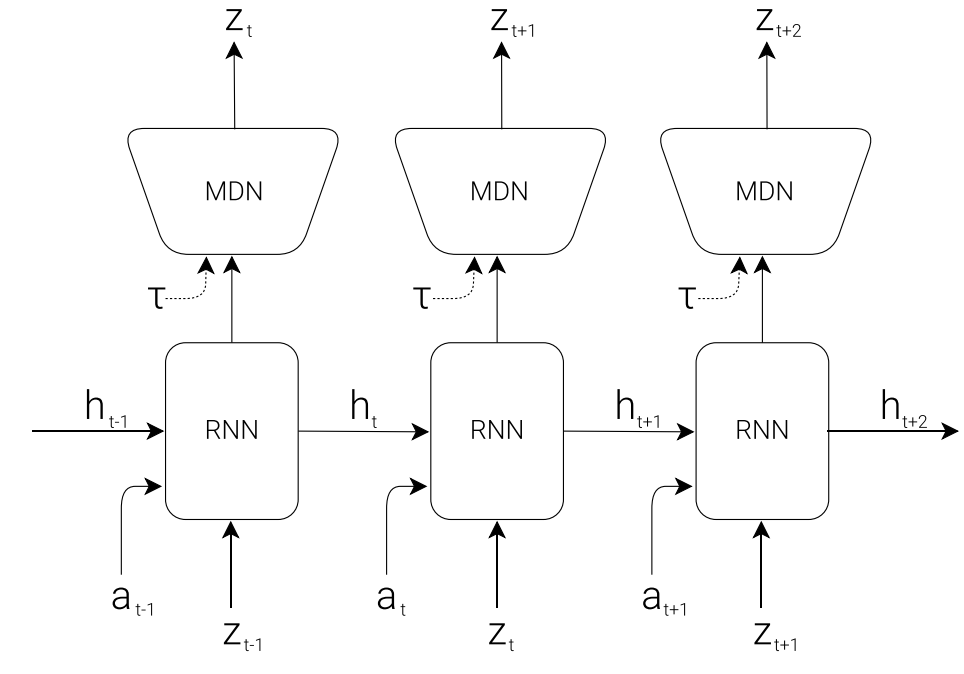
\includegraphics[width=0.75\columnwidth]{sections/4rlopt/images/mdnrnn.png}
  \caption[Temporally unrolled MDN-RNN]{Structure of an unrolled MDN-RNN. The MDN outputs the parameters of a Gaussian mixture distribution used to sample a prediction of the next latent vector $z_{t+1}$, the MDN is controlled by the temperature parameter $\tau$.}
  \label{fig:rl:mdnrnn}
\end{figure}

By combining the mixture density and recurrent networks, we can use rollouts of the environment sampled using a random agent to train the combined network, called an MDN-RNN. We use the network to model $P(z_{t+1}~|~a_t, z_t, h_t)$, where $z_t$, $z_{t+1}$ is the latent state at the times $t$ and $t+1$ respectively, $a_t$ is the action taken at time $t$, and $h_t$ is the hidden state from the RNN network at time $t$. Figure \ref{fig:rl:mdnrnn} shows the combination of the RNN and MDN networks and how we calculate the predictions of the next latent state in sequence.

A constraint of using RNNs is that they expect a fixed sized input sequence. However, in our work, both the shape of the latent state tensor, and the number of actions performed by the agent in a rollout is variable. As such, we employ a common approach to mitigate this problem is by prepending zero values to the input sequence until the desired length is reached, commonly referred to as padding. After performing inference on the model and retrieving the predicted state, we mask the results based on the input padding to ensure we only use valid predictions to select the next action using the controller.

Furthermore, after training the world model, we must train an agent (or controller) to perform actions in the world model and learn to take optimal actions that maximise reward. During inference of the world model, we use a softmax layer which outputs $\pi$ in the form of a categorial probability distribution. We can sample the distribution under the Gaussian model parameterised by $(\mu_i, \sigma_i)$. Similar to the method of knowledge distillation, we incorporate the temperature $\tau$ into the softmax function which allows us to control the stochasticity of the agent during training of the controller.

$$
y_i(\mathbf{x}|t) = \frac{\exp\left( \frac{z_i(\mathbf{x})}{t} \right) }{\Sigma_j \exp \left( \frac{z_j(\mathbf{x})}{t} \right) }
$$

\subsection{Action Controller}